\chapter{Sensing in the Built Environment}

Buildings consume nearly 40\% of the total energy produced in the United States and 72\% of the electricity.  Similar figures 
have been recorded in other industrialized countries~\cite{buildings_study}.  Furthermore, studies show that they waste from
30-80\% of the energy they consume.  With specter of global warming and the continued decrease in the cost of storage and 
communication, buildings have become a major target for improved energy efficiency.

Large commercial buildings typically contain thousands of sensors embedded in them which report periodic readings to 
a centralized system called a building management system.  Typically these have been installed for supervisory control and
centralized observation of the building.  The kinds of sensors installed including temperature sensors on the thermostats,
valve position meters and actuators on pipes, pressure sensors in the vents, temperature sensors on the vents and pipes, etc.
These readings are combined with a graphical interface for building managers to visually locate them according to their location.
The interface also allows them to visually inspect and quickly try to diagnose a problem, typically in response to occupant
complaints.

Although these systems have been revolutionary from a building management perspective, they lack many fundamental components for
truly enabling sophisticated analysis -- the kind of analysis that is needed to understand how the building is performing
and will perform in the future.  Also, building practices for software-driven building systems serve more as guideline than
 as a standard.  This presents major challenges with respect to software re-use and scalability.  In this thesis
we will discuss the how we address these challenges through architectural design choices and analytical metholodology.  
The achitectural choices reconstruct the software layer that sits on top of existing building management systems and presents
a unified interface and standard API for analytical and control building applications.
The analytical methodology offers a general approach to verifying the construction of point names -- the naming scheme for 
sensors distributed throughout the building.  Both set a foundation for ongoing and future work.

The thesis is presented in the context of building systems and building-related applications.  We draw out the fundamental 
components in our analysis and design and discuss where it fits in the broader context of prior, computer science related,
literature.  In the next section, we describe the state-of-the-art practices followed by vendors of building information systems.
We describe the architecture features and design principals both implicitly and explicitly implemented into these systems.
We present the pros and cons of these decisions and their implications and include a high-level description of our approach.
Later chapters delve more deeply into the implications of our design decisions.

\section{Tightly Integrated Building Information System Architecture}
% Nearly three-quarter of building 100,000 square feet or larger, have a building management system (BMS) installed.  
% A BMS typically consists of thousands of sensors, distributed through the internal spaces in the building, periodically reporting 
% the state of the environment and the health of the individual sub-systems.  Their primary use is to maintain and diagnose problems
% in throughout the building, as they are reported to the building manager.  However, recent interest in energy has motivated the 
% expanded use of their data-gather capabilities in order to uncover opportunities to improve their overall performance, increase the
% lifetime of the building, and make buildings more comfortable its occupants.

% The suite of software available to contractors and architects is quite fast.  Ranging from pure simulation engines, such as 
% DOE-2~\cite{doe_2} and EnergyPlus~\cite{eplus} to offline analytical packages that combine the strength of statistical analysis
% with building models~\cite{osisoft}.

The first building information systems became commericially available in the 1970's ~\cite{gardner1987energy}.  
Historically, building management 
systems were constructed as a collection of control loops, which progressed from pneumatic to analog to digital.
These control loops largely form the foundation for the design decisions made in building information systems.  
This section gives a quick overview of the architecture bottom-up and describes how each stage is built around
the concept of loops and supervisory control.  We then describe some of the short-comings of this architecture
and give an overview of how we address it in a system called StreamFS -- described in more details in
the remaining chapters.

\begin{figure}[t!] %htbp
\centering
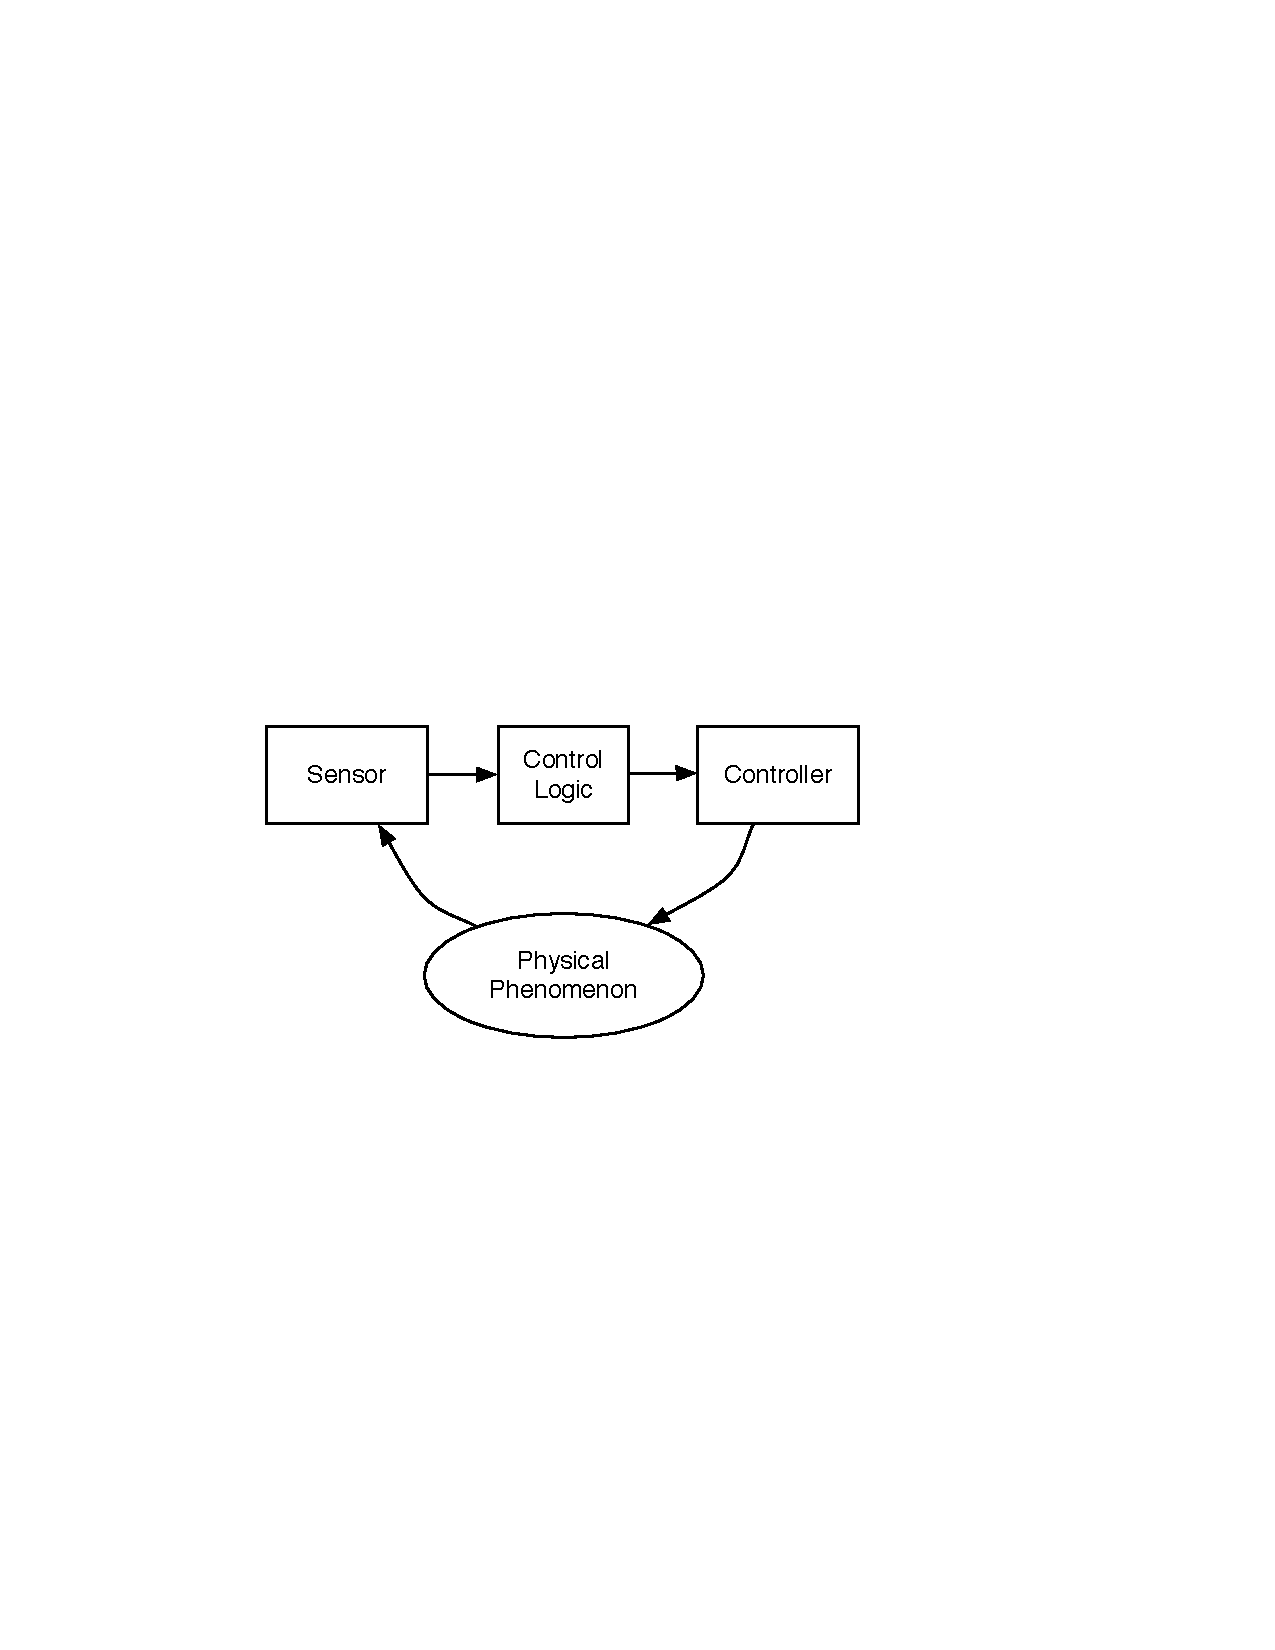
\includegraphics[width=0.50\columnwidth]{figs/control_loop}
\caption{General building control loop.}
\label{fig:control_loop}
\end{figure}

\subsection{Control Loops and The Outstation}
\label{sec:control_loops}
Each loop is defined by a control domain consisting of a sensor, an actuator, and a control mechanism.  The control mechanism
become logic based when signals from sensors moved to the digital domain.  However, the basic control principal was based
entirely on local control loops, with the implicit assumption that these loops were largely independent of one another.
Figure~\ref{fig:control_loop} shows a high-level control loop.  For example, the temperature control loop has a temperature
sensor as the input and uses the temperature set-point parameter to decide when and which actuators to activate.
For temperature control this actuation controls the the valve that lets cool air into the space.  This causes the temeprature
to fall until a lower-bound is reached and the control logic is activated again.

The figure also shows the basic structure inside an outstation.  An outstation is a box that contains up to several control boards, each
wired to one or more sensors and one or more actuators.  The outstation is typically close to the sensors and actuators (in the same room)
and contains all the control logic for the local plant.  Inside the control logic there is a CPU and some memory.  The memory
contains the control program and some space for sensor readings.  It is directly wired to the sensors and actuators through
a series of buses and shown in Figure~\ref{fig:control_box}.

\begin{figure}[t!] %htbp
\centering
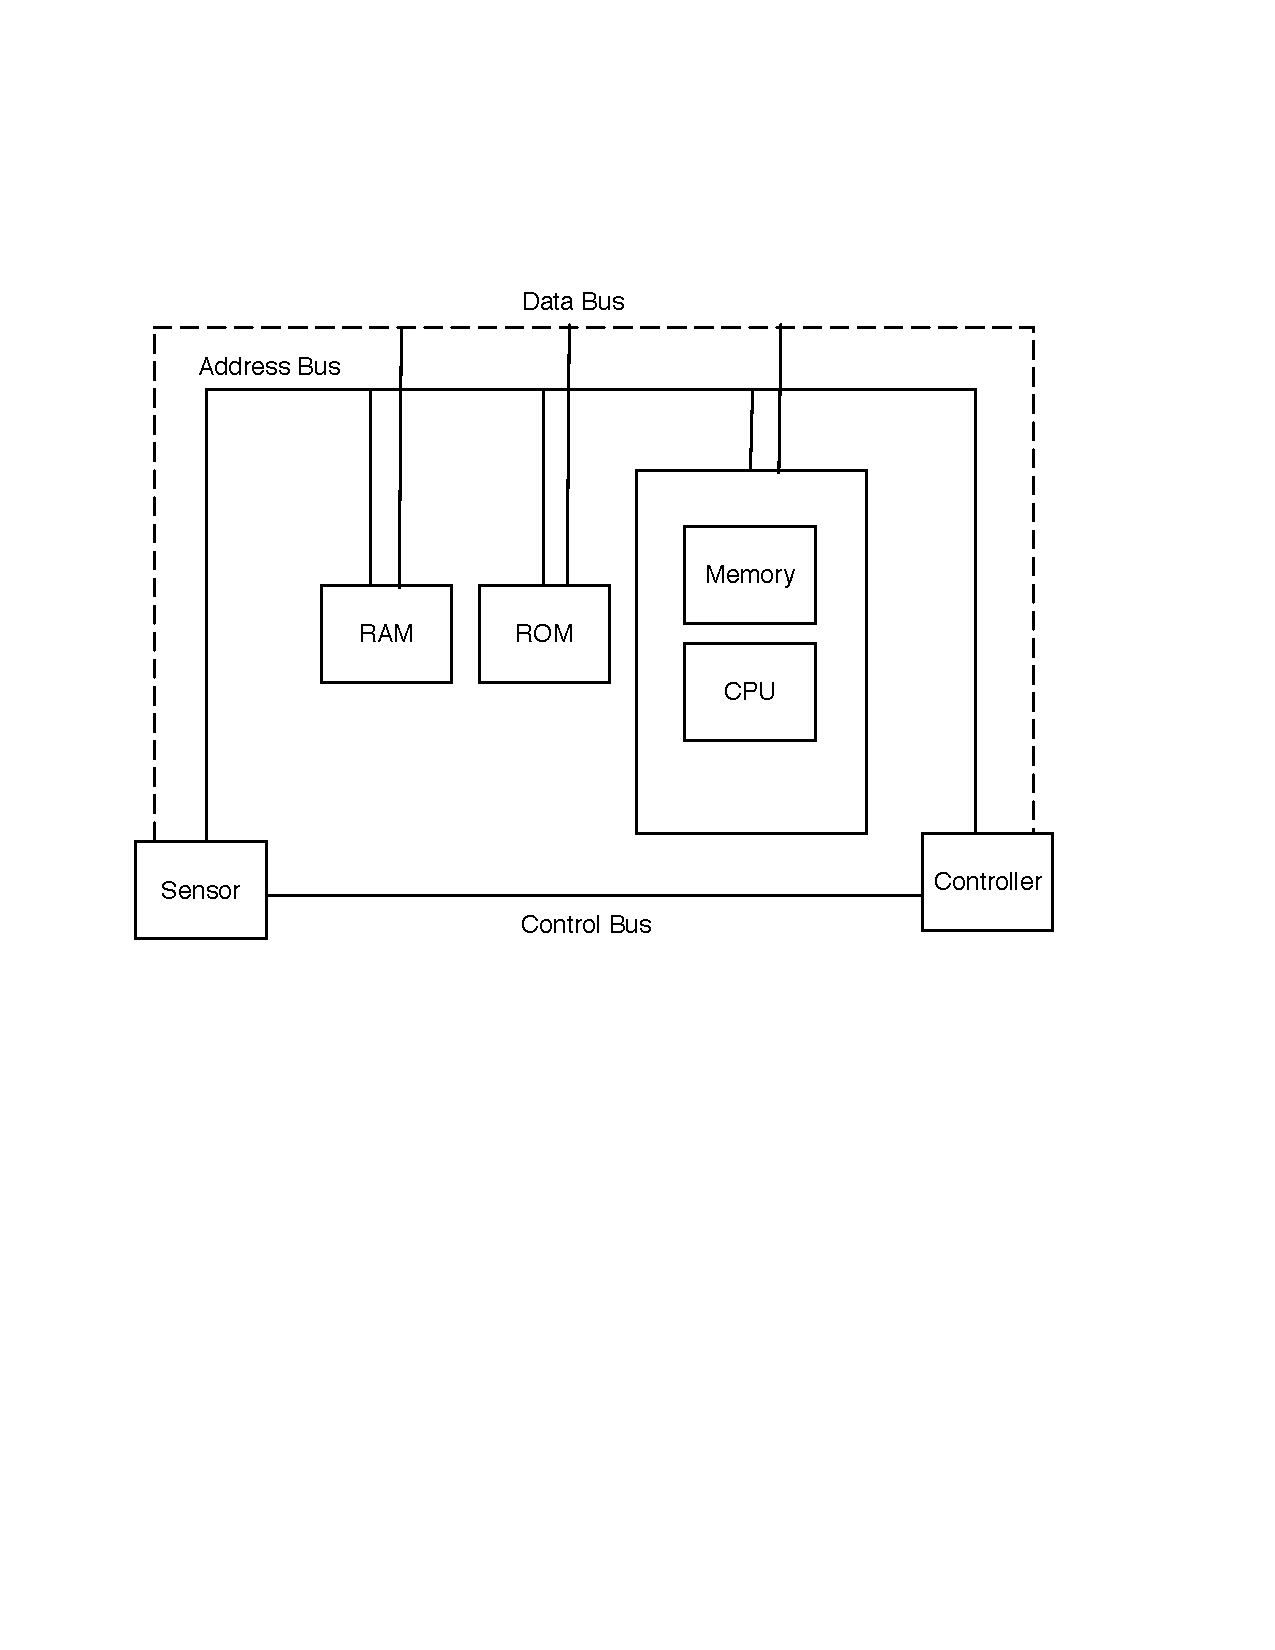
\includegraphics[width=0.50\columnwidth]{figs/control_box}
\caption{High-level control board architecture.}
\label{fig:control_box}
\end{figure}

As readings from the sensors are taken, they are placed in RAM.  The amount of RAM is limited and can get filled up, so it is important
to schedule periodic collection tasks from the central station -- the building management system (BMS).  The control logic is typically
written in ROM and can only be changed by the vendor.  The input parameters are set at the BMS and they dedicate the operational dynamics
of the control scheme in reaction to the input~\cite{BMS_book}.
Outstations are distributed through the building and are essentially running independent of one another.  In order to enable centralized 
monitoring and control, they are networked together and report some of the sensor readings and control-logic state to a central outstation.

\subsection{Central Outstation and Communication Protocols}
The central outstation is typically a Microsoft Windows-based PC connected to the outstation through either RS-485/modbus or ethernet.
The user interacts with the system through a graphical interface, constructed from the schematics for the building or the schematics
for the component in the system that is being monitored.  The BMS running on the PC communicates with the outstations through either a 
proprietary protocol or an open one like BACNet~\cite{Bacnet} or LonTalk~\cite{LonTalk}.

\begin{figure}[h!] %htbp
\centering
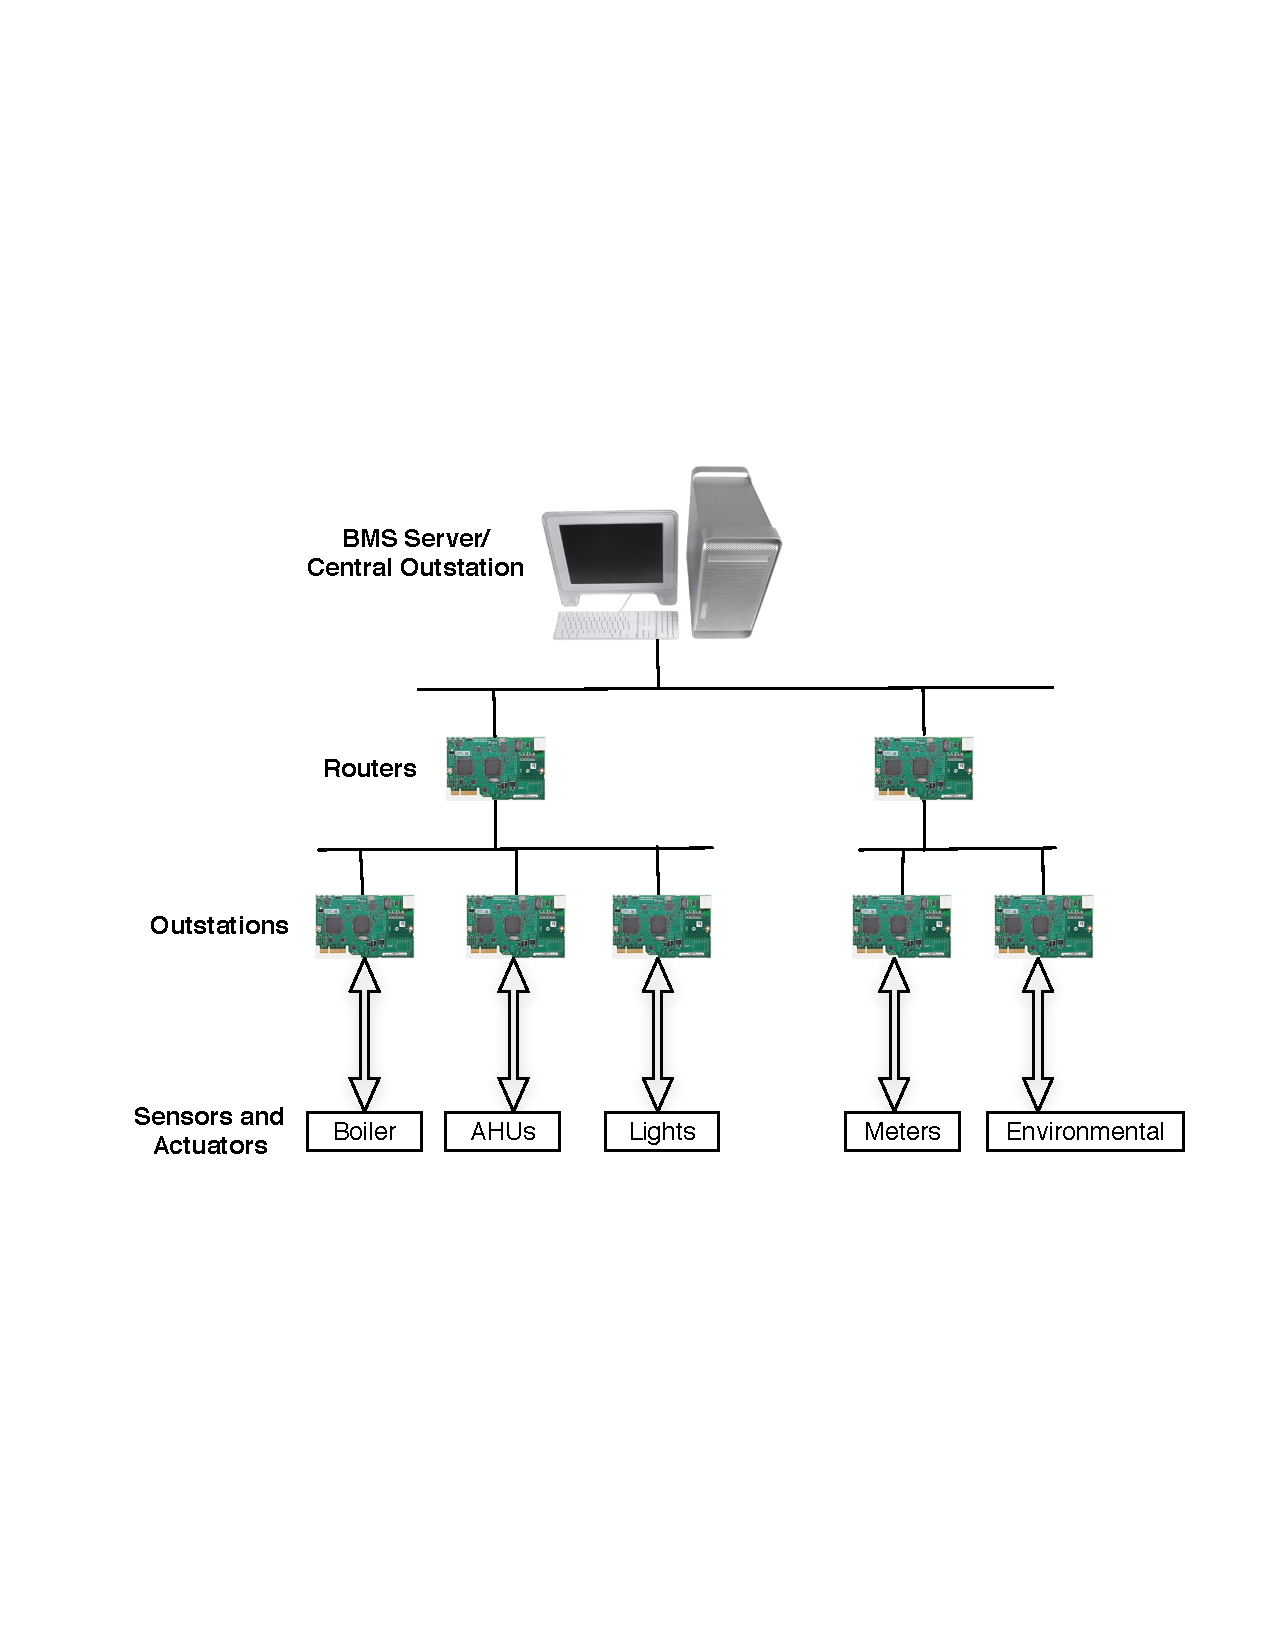
\includegraphics[width=0.50\columnwidth]{figs/BMS_network}
\caption{High-level control board architecture.}
\label{fig:bms_network}
\end{figure}

Both protocols define both a wire protocol and packet structure for communicating with the outstations.  From these there's a high-level
structure for the individual points throughout the system.  A point is a sensor/actuator or another kind of object, like a schedule object.
BACNet exposes the notion of devices as a collection of different types of objects.  Each object contains a set of properties that can 
be read and/or written.  A device is identifyable through a name or address on the network, each object has a unique identifier and is one of
many types -- such as input, output, value, analog, and many others~\cite{Bacnet}.  

These protocols also provide a protocol for discovery and read/write.  Each [device, object name/id, property name/id] tuple forms a name.
This name is typically what is exposed by the protocol to the application.  All the names are set by the vendor and the graphical interface, 
constructed from the building schematics, is also designed and constructed by the vendor.  The building manger is the primary user of the system,
so rather than expose the underlying protocol, he/she interacts with the building via the graphical interface.

In order to interact with the underlying sensor and actuator layer, the application must use a stub that communicates directly with the 
sensor/actuator through the BACnet stack.  Services treated similarly to sensors/actuators.  They are represented as a collection of 
objects with readable/writable properties.  An example service that is provided in BACNet is  \emph{WhoIs} and \emph{EventNotification}.
The former is a broadcast service that is used for discovery of other objects, the latter is used for setting alarms on the sensor data that
are reported by the BACNet enabled devices on the network in the outstation layer.  There are many other types of events that are supported 
and over 50 types of object types in the baseline protocol, which is extensible.  Device and object names that are added have no restriction
on either the number of characters (specified by the vendor) or the encoding.


\begin{figure}[t!] %htbp
\centering
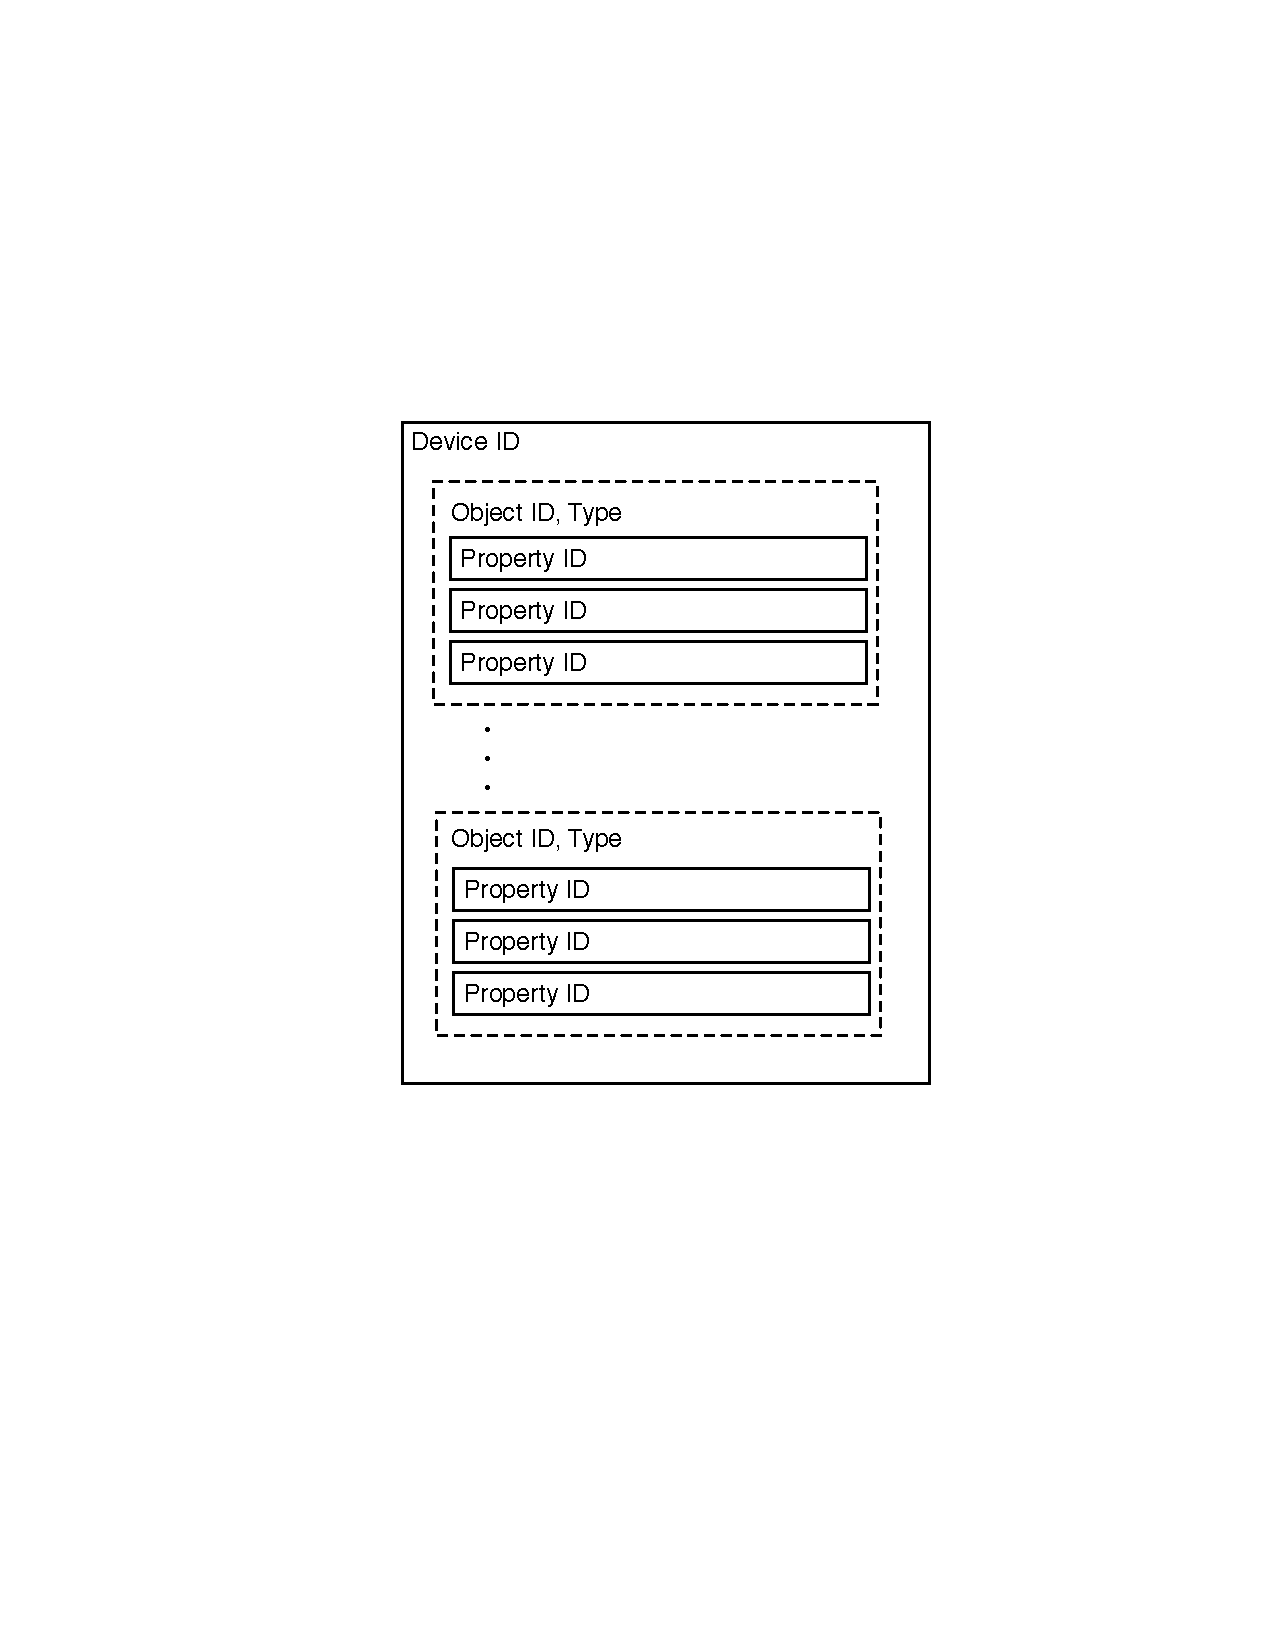
\includegraphics[width=0.25\columnwidth]{figs/bacnet_device}
\caption{BACNet device example.}
\label{fig:bacnet_device}
\end{figure}

% \section{Current and Future Building Applications}
\section{From Supervisory Control to Application Development in Buildings}
Building information systems were built as tightly integrated silos, where the main application is the graphical user interface.
Features for interoperability were designed at two interface layers: 1) the protocol layer and 2) data export features in the 
graphical interface.  The protocol layer -- we focus on BACNet, but the similar features exist in othe protocols, such as LonTalk --
provides services for enabling devices to talk to one another through the network.  Several features were explicitly designed around
the notion of interoperabilty, namely trending, scheduling, management services, alarms and events, direct sharing.  The graphical
interface layer is mainly focused on providing periodically reports, typically in the form of a comma-separated value file, which
contains point-name information and time-value pairs of data.

Historically, the extent of interoperability objectives has included mainly the introduction of new devices onto the network or
the exporting of data for other software program to use for analysis and report generation.  Building informtation systems themselves
were constructed mainly to support the in-time management and supervisor control of the building.  Analysis does not 
extend far beyong univariate plotting and individualized assessment of equipment and control not far beyond manual parameter tuning
of hard-wired control logic at the outstation.

Over the last few years, however, there has been in increased interest in energy management and comfort as a primary objective 
in the design of new building applications~\cite{}.  Moreoever, there is a broad interest in having buildings participating in hierarchical, 
global control schemes that optimize the performance of the grid in response to renewable source penetration and its inherent 
generation volatility~\cite{}.  Model predictive control has introduced new ways of controling the components in the building
to make them more energy efficient~\cite{mpc}, there is an interest in performaning dynamic, real-time analysis of building health
and efficiency~\cite{dynamicLeed}.  There has even been interest is improving the visibility of the state of the building to the 
occupants through various modalities, including touch-screens~\cite{} and mobile phones~\cite{andrew_lighting, buildsys1, buildsys2}.  
These are other emerging applications
have pushed the boudanries of the capabilities of building information systems and a re-design must be considered.

% \subsection{}



% The notion of applications in building has been around for some time, but almost exclusively in research.  The bulk of commercial
% applications revolve around better visualization of building data through the web.  Recently~\cite{andrew_lighting, buildsys1, buildsys2},
% there has been to work to expand the notion of building applications to include both visualization \emph{and} control.  Visualization, itself,
% has broadened its reach to include personalized, aggregate, real-time views of energy consumption.

% \subsection{Code Compliance}
% The primary use of simulators on the market, is for code compliance.  There are building codes that are mandated by each state and across
% the nation, that dictate the construction and health of newly constructed buildings.

% \subsection{Energy Auditing}
% Energy auditing is now seen like an application in buildings.

% \subsection{Retrofitting}
% Retrofits refers to the addition of new technology or the replacement of old technology to improve the performance of a system.  In the case
% of buildings, this means improving some aspect of the construction of the building in order to improve its performance.  Often, simulations
% are used to test the effects of retrofits in simulations and made decisions about whether or not to invest in a retrofit.  For example, 
% the physical construction and replacement of the windows, the addition of sky lightings, the addition or replacement of HVAC components, are
% all examples of retrofits that can be tested in simulation before they are purchased.



% \section{BMS Design Flaws for Supporting Future Building Applications}
\section{BMS Architectural Shortcomings for Supporting Emerging Application Development}

\begin{figure}[t!] %htbp
\centering
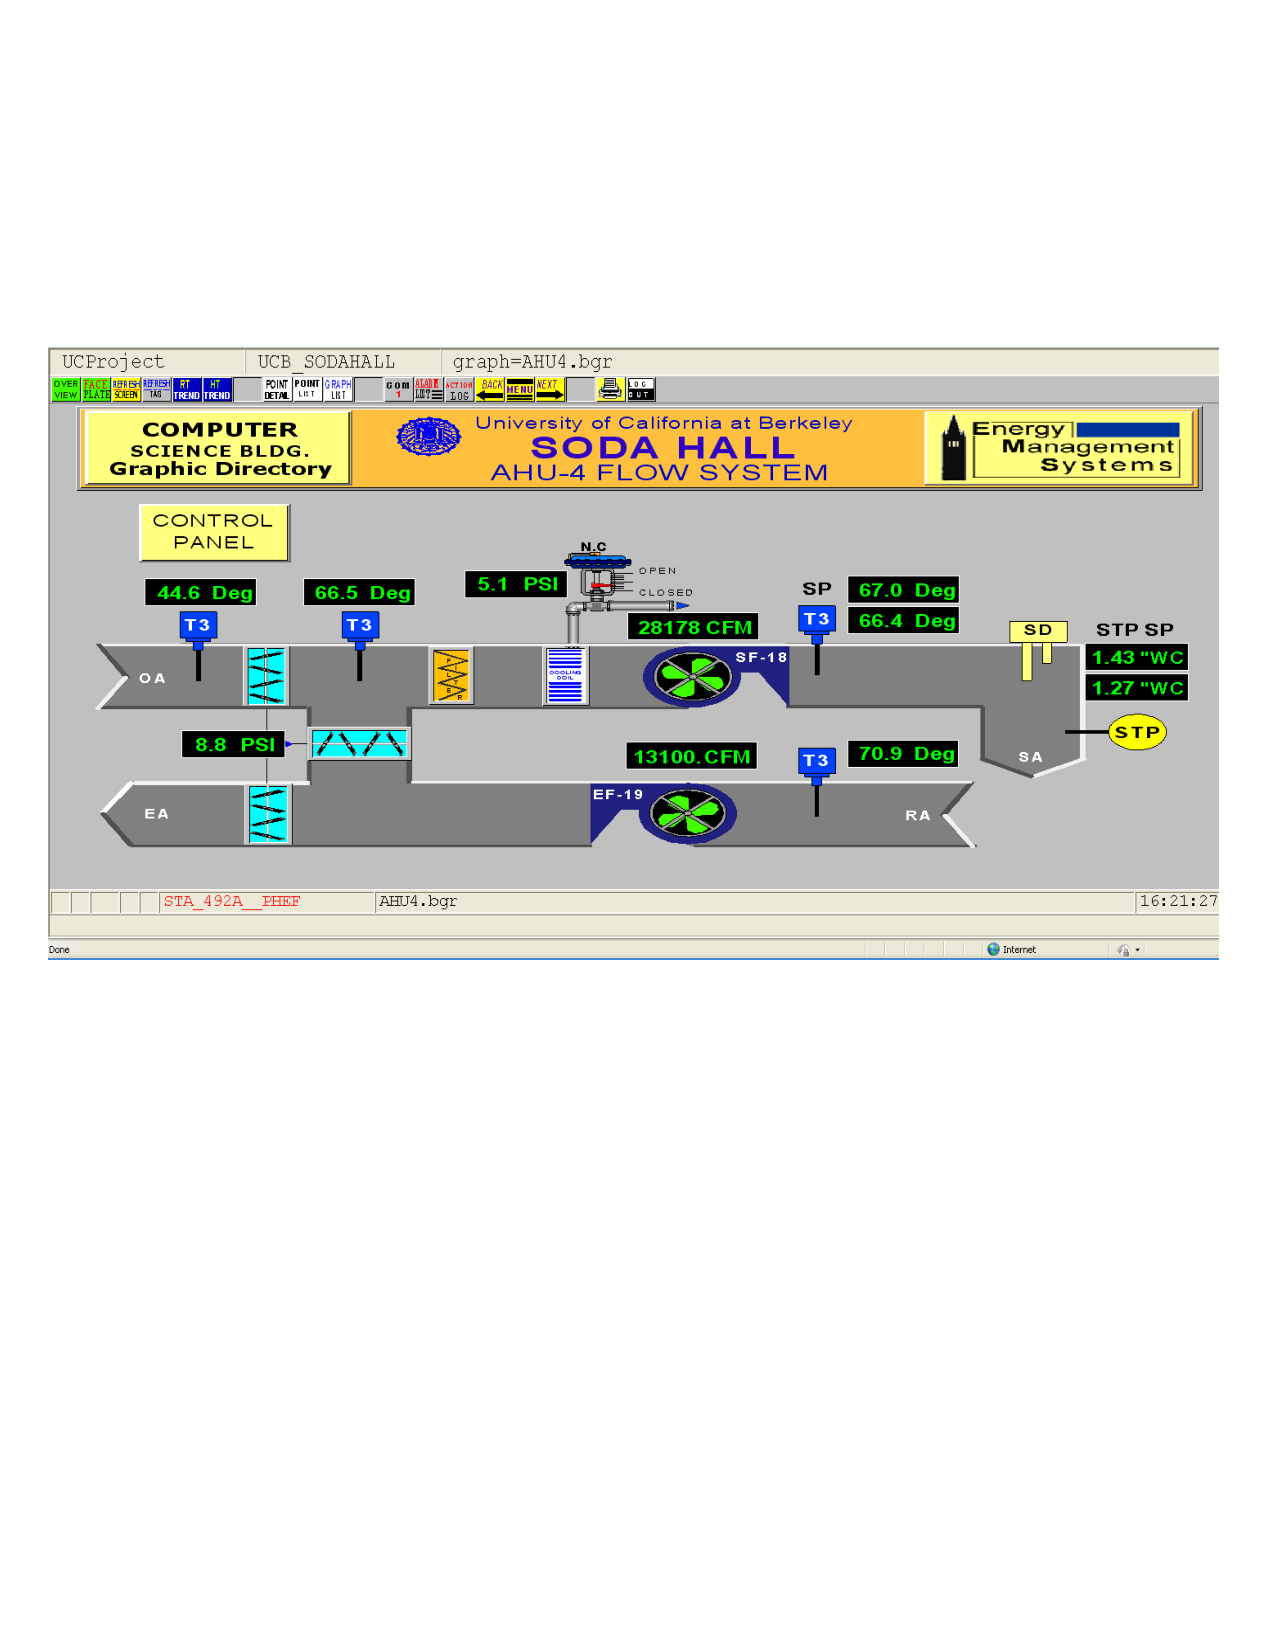
\includegraphics[width=0.75\columnwidth]{figs/soda_bms_screenshot}
\caption{Screen shot for the Soda Hall Building Management System Interface.}
\label{fig:soda_bms_screenshot}
\end{figure}

% In this section we dissect the current architecture in the context of current and future applications
% for buildings.  The first two describe how the current architecture is used to provide the intended service
% that these application provide.  The latter two are emerging applications that we would like to available
% throughout the entire building stock.  We will see, however, that these are very difficult to build at scale
% and we pose the question ``what is missing in the current architecture to enanble the system properties that help
% support these and other emerging applications?''.  Through close inspection it will hopefully become clear that
% the current architecture is fundamentally flawed; built largely to support a small set of vendor-specific
% applications and not much else.

In this section we dissect the BMS architecture and closely examine how well it can support broad application development
in buildings, rather than the single supervisory control function it supports today.  We examine the architecture in the context
of 4 potential services with distinct operational requirements that need to be supported.  The first two services that 
are offered today and enabled by the BMS.  We describe how emerging requirements are driving the evolution of these
services and how BMS's are struggling to meet the new requirements due to limitations in their architectural design.
The next two are emerging services that BMS's cannot support today.  We describe which architectural components must be included
or how current components must be modified in order to support these.  We also make the broader argument that 
building systems should be built to support a much wider range of applications that we cannot currently anticipate.
We will show why this requires a fundamental re-design and propose an architectural composition for such a system.
In the rest of the thesis, we will examine an instance of our architecture and describe the challenges in realizing
the use and effectiveness of our system in real building deployments.

% while the latter are potential applications we imagine will be supported in future
% smart buildings.  Through this exercise, we build our argument for a systematic re-design of such systems and propose
% a set of necessary architectural components necessary to enable and support emerging applications.

\subsection{Monitoring and Supervisory Control}
The primary objective in the design of building information systems is for centralized monitoring and supervisor
control.  Control algorithms are left ``to the expert'' and embedded in the outstation control board.  The intended
user of the system is a building manager -- a user whose expertise is more high-level than control-algorithm or system specific.
The manager is expected to monitor the health of building systems and quickly diagnose problems when they occur.  The tool
is mainly in place to save the building manager time; and it is very effective at doing so.  The extent to which 
the building manager is making control decisions is altering control algorithm paramter setting through
the building management interface itself.  Even these decisions typically go through the vendor, through consultation.

Figure~\ref{fig:soda_bms_screenshot} shows a screenshot of the BMS in Soda Hall at UC Berkeley.  This specific image
captures a schematic for one of the air handling units.  It shows the various sensors embedded in different locations
on the component -- on either side of the supply/exhaust fans, temperature sensors at the supply/return sides of the
air ducts and the inlet vent, measuring the outside air temperature.  Accompanying real-time readings are juxtaposed
by the sensor image.  The user can double-click on the sensor or reading to get more information about that particular 
measurement point.  For example, if you double-click on a temperature sensor, it will give you the exact name of the 
point and accompanying information about related points, such as the set-point, which effectively drives the behavior of 
the underlying system.  If an occupant makes a complaint about not getting any air from the vents, for example, the 
building manager can find the screen for the vents that serve the room the occpant is in and observe the current
pressure readings or look for value-based alerts on any of the readings, typically displayed on the same screen.
If there is a malfunctioning component or something stuck in the vent, the readings should ``look off'' to the building 
manager.

If the problem recurs often, the astute building manager may be able to characterize the fault through a series of alarms.
They can be proactive about finding and fixing the problem(s) before they occur.  Alarms can be set through interaction
with the graphical interface, in much the same way that a lookup on the measurement point occurs -- by double-clicking on 
the point in question and following instructions for setting an alarm.  In some cases, the problem may be driven 
by a faulty setting and adjustments can be made to the control parameters through the associated control points.

The scope of control is limited to specific control loops.  Recall our discussion of control loops in section~\ref{sec:control_loops}.
The building manager can, typically with the help of the vendor, decide on the best control strategy setting.  If the control
strategy cannot be met, due to flaws in the control algorithm itself, the vendor may step in and re-image the controller
at the outstation and expose the necessary parameters through the graphical interface.  These kinds of changes are rare
but do happen occassionally and can be somewhat expensive, since the cost is not typically included with the purchase
of the system.  Because of the cost, the decision is typically made after close inspection and analysis, which a typical BMS
enables.  For example, the sense/control points in question may be placed in ``trend'' mode.  This means that readings
from those streams are stored in the local memory buffer at the outstation for some period of time.  If a report is specifically
set up at the central system, a report period if also associated with the point, allowing the saved points to be drained
from the local buffer at the outstation.  The points are then placed in a file for observation and graphing by the 
building manager.  Time-dependent inspection of the behavior of any of the control-loop related points can be examined.

Although this feature is not necessary in order to change control paramters, it is useful for observing how parameter changes
affect the behavior of the system.  The building manager can, in principal, experiment with different setting and allow
empirical observations to guide her future decisions.


\subsection{Energy Auditing and Building Modeling}
Recently there has been renewed interest in the energy consumption of buildings.  In particular, several studies~\cite{BuildingEnergyData,
MITBuildingScience} show that buildings consome a large fraction of the energy produced in the United States and that as much
as 80\% of it is wasted.  As such, there has been an emergence of several companies and services for assessning the health of
commercial buildings with respect to their energy consumption.  Organizations such as LEED~\cite{Leed} provide certification of 
buildings, specifically rating the energy efficiency of the building.

Building modeling has been part of building science for quite some time, with systems such as EnergyPlus~\cite{EnergyPlus}.
EnergyPlus and simulators like it are part of a larger ecosystem of software for modeling various aspect of the operation
of the building.  They allow the designer to construct detailed models of the building, from construction to usage.  You can
model everything from the material, location, zone-based usage (office building, bathroom, storage room), window size and its
construction, etc.  There are different types of LEED certification, but typical certification requires the submission of the detailed
model and the results of various energy-related metrics, aggregated over seasonal time intervals to attain LEED certification.

Detailed model construction can take several months and in order to ground the underlying model in empirical performance data
typically a modeler will use the data obtained from the building's BMS.  Most vendors provide a way to export the point-related 
trended data.  Complex models can be built using this information.  The file export feature in combination with the ability to 
``trend'' points provide an interface mechanism for these and other kinds of applications that need to make use of the data.

Another option is to obtain the data directly from the system through the network.  Third-party vendors provide systems that 
will join the building network of devices and eavesdrop of the readings and traffic being reported to the central server.
This is the only way to obtain truly real-time readings from the sensors on the network.
Typically BMS vendors do not like this since they may generate too much traffic and overwhelm the network because of congestion.
Although not fundamental, it is a common concern in buildings today.  Many buildings use RS-485 rather than ethernet and there is
a general, albeit unfounded, concern that the network will become overwhelmed if all the points are trended and report at the same
time.

Building modeling and real-time analysis have been separated because of these constraints.  The constraints are largely not
fundamental, but the current architecture is simply not designed to provide real-time readings for \emph{all the points, simultaneously}.
Also, it is clear, even from the fairly simple workloads generated by these analysis applications, that a history of readings
is needed.  BMS's, as currently designed, require the end-user to manage the history of the data point individually.
When BMS's were first designed, there were certainly concerns about bandwidth and storage limits.  However, today those concerns
are a non-issue.  A few hundred bytes produced on the order of a few minutes, even from several thousand sensors is simply not
that much data.


\subsection{Holistic Building Optimization}

\begin{figure}[t!] %htbp
\centering
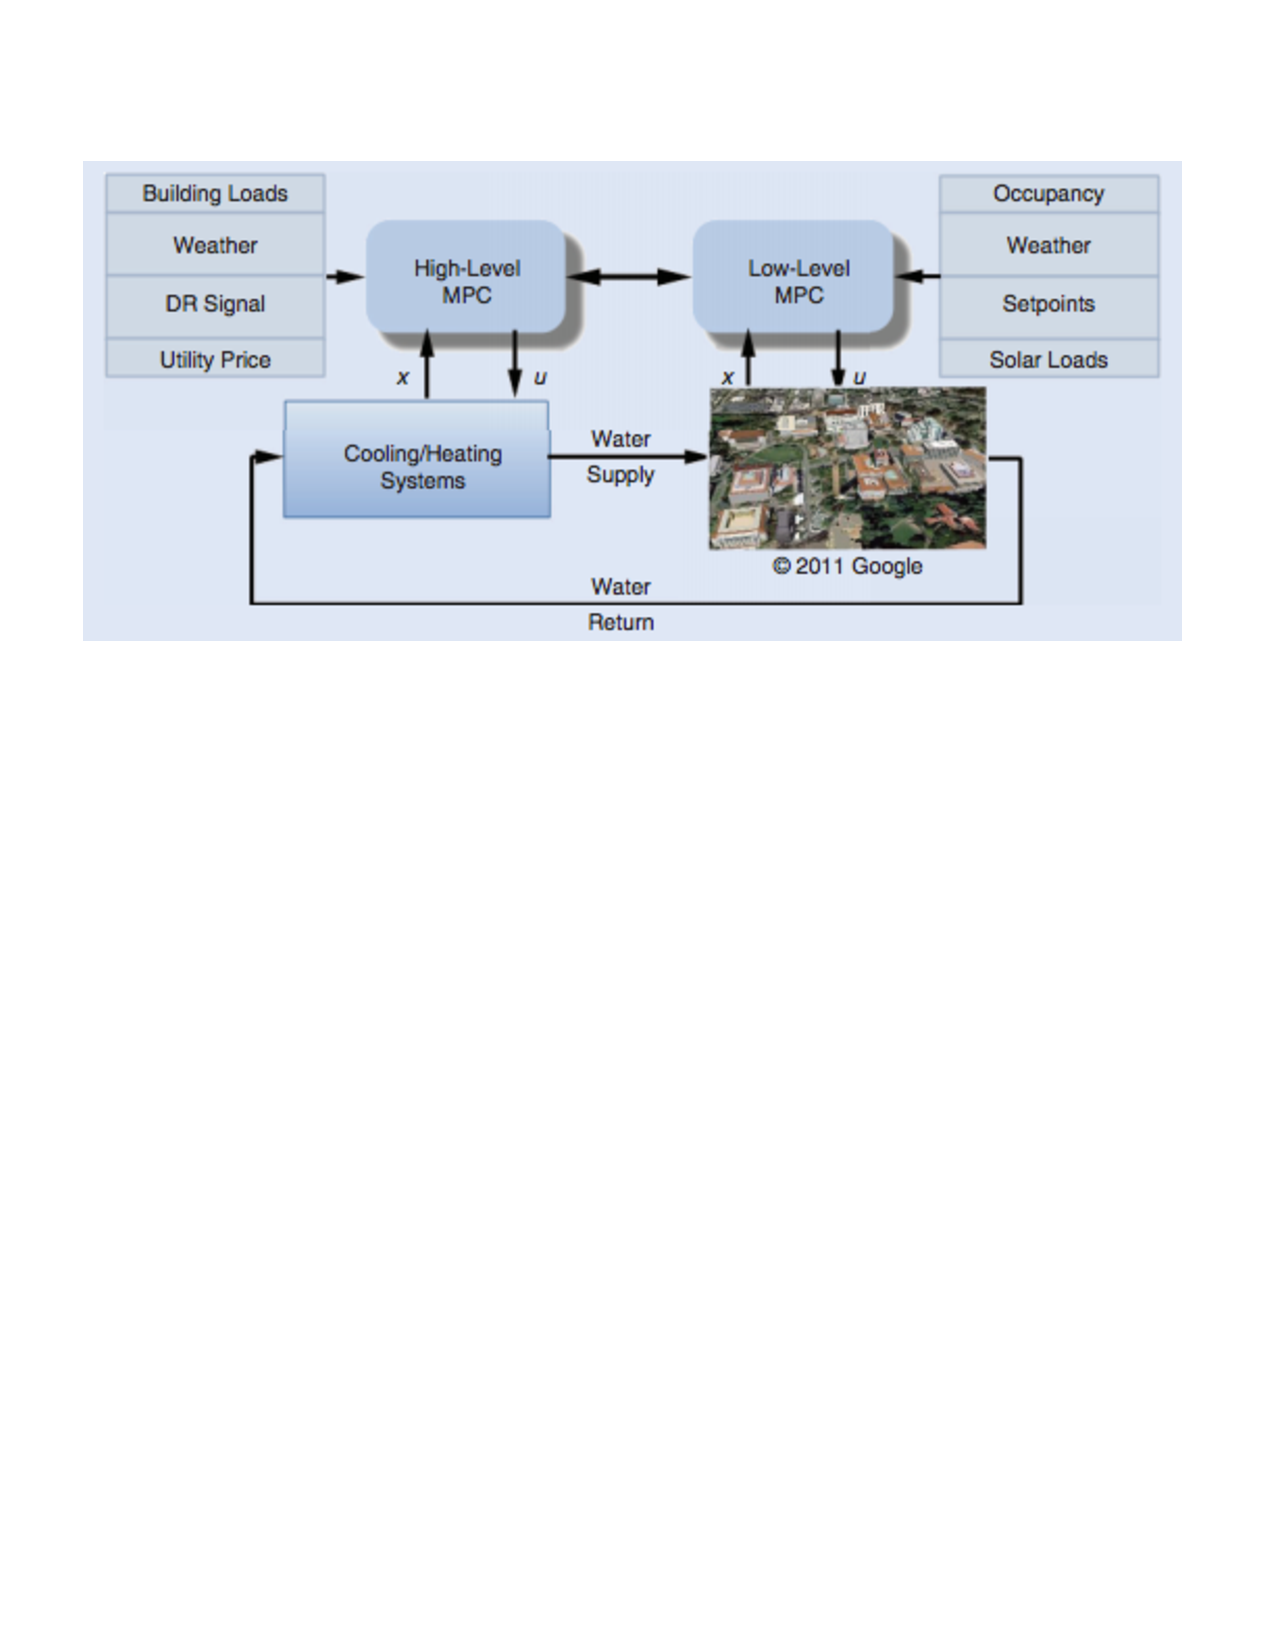
\includegraphics[width=0.75\columnwidth]{figs/mpc1}
\caption{Emerging Application: Hierachical MPC for a stock of buildings.}
\label{fig:mpc1}
\end{figure}

An emerging class of applications, is in holistic control of the building using a new technique called model-predictive control~\cite{MPC}.
Rather than rely on specific changes to control logic at the local-loop level, MPC techniques observe and learn a model
of the behavior of a components, multiple components, or the whole building, based on the historical data.  Once the model is learned, 
constraints can be specified to drive the behavior of the system to an optimal region in the tradeoff space; solving it as 
a constraint optimization problem.  Figure~\ref{fig:mpc1}, reproduced from~\cite{MPC}, shows an example of the how MPC combines 
several points in the building to control the building.  Essentially it decomposes a large optimization problem into indivial control 
decision to be made at the control-loop level.

In order to build this application, the set of necessary points must be mapped into the process.  The user, setting up the problem,
must connect the right data streams and control points to the algorithm by either manually going through the schematics or
locating the schematic representation in the BMS graphical interface.  There is no query interface and it requires that you sit
with the building manager or vendor in order to set up the trending, reporting, and enable the necessary control permisions.
The process is time consuming and \emph{does not scale}.

Although the method is very useful and has yielded excellent results, it is difficult to replicate.  The code and setup must be 
customized for each building or stock of buildings it is set up on.  This lack of generalizability and scalability is missing
in the current state of the art of building information systems.  In most cases the representation of sensor/actuator association is 
implicitly represented in a combination of the schematics, the graphical interface, and the point name.  Moreover, all
three of these change from building to building.  It is fundamentally difficult to generalize.  Buildings are treated as one-off constructions
and their associated digital information has historically followed the same principle.


\subsection{Personal Energy Viewer}
\label{sec:mobile}

\begin{figure}[h!] %htbp
\centering
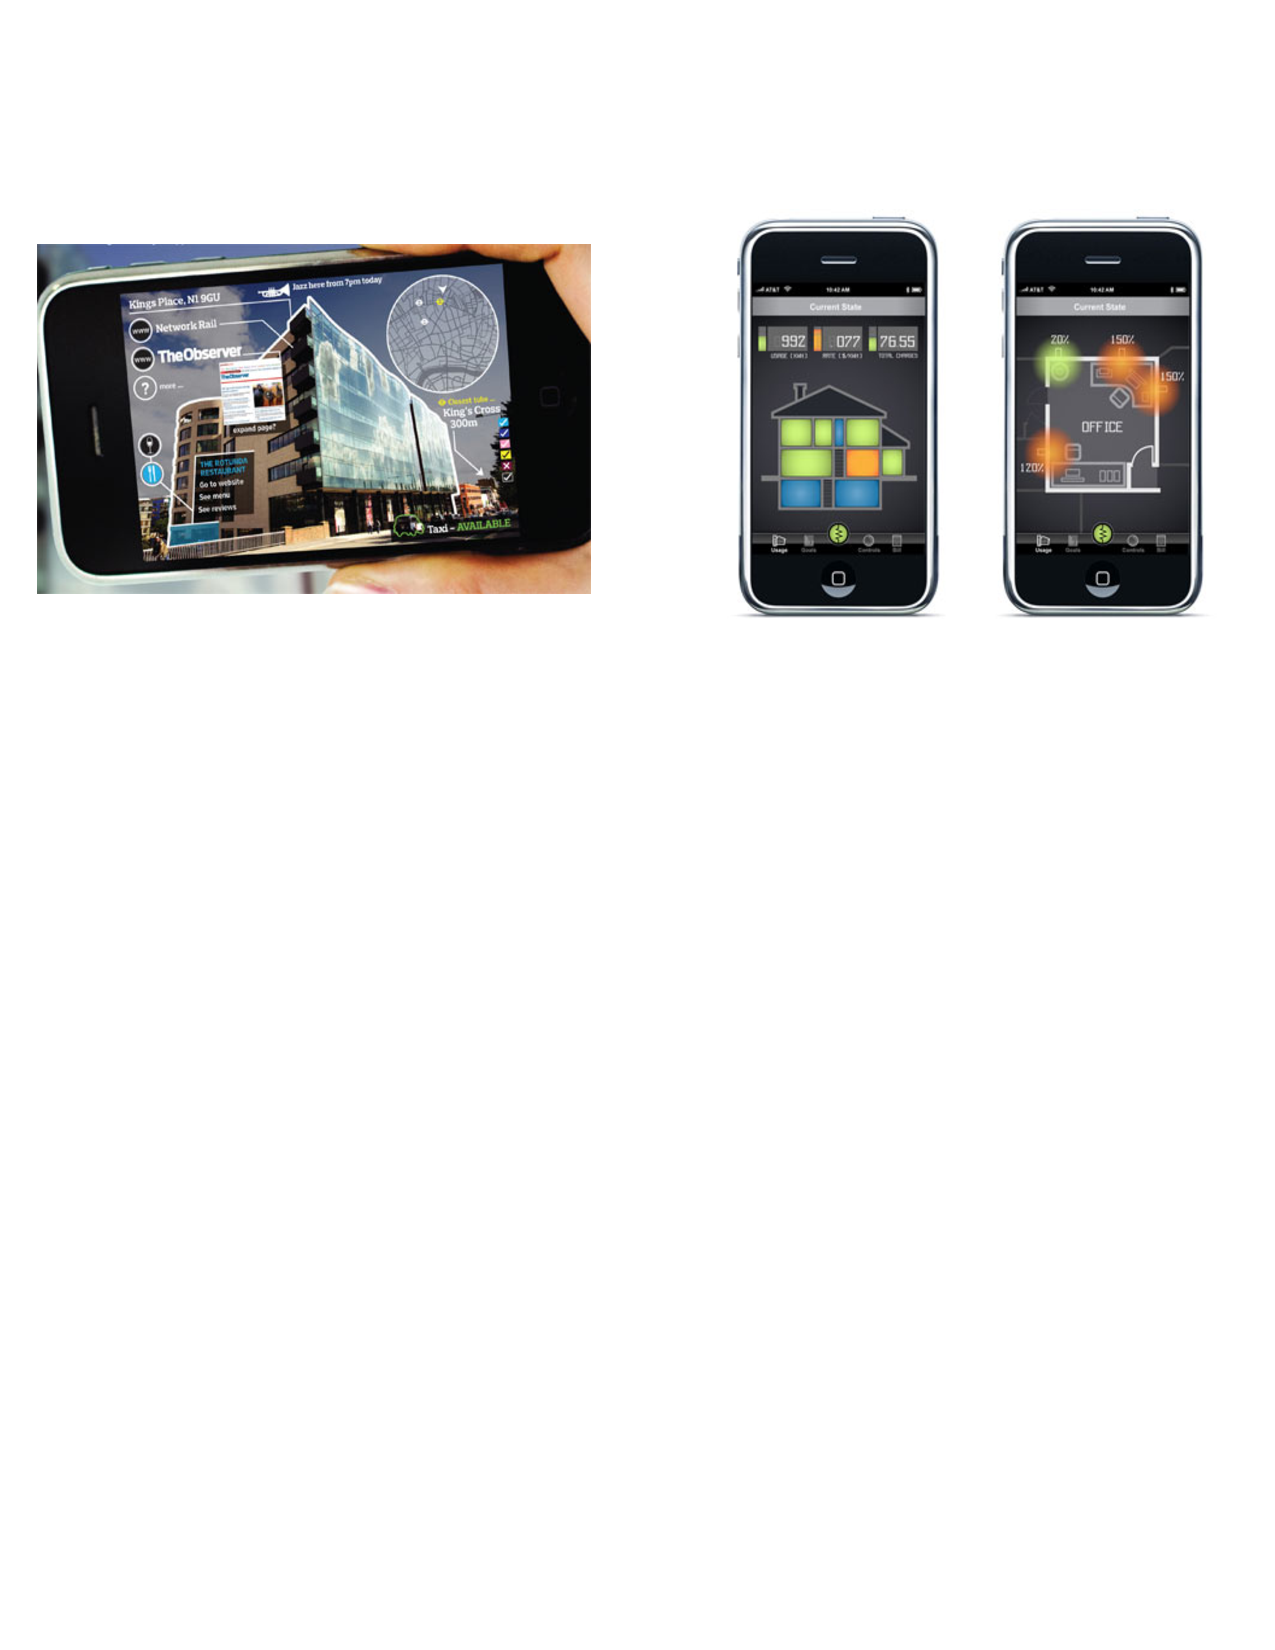
\includegraphics[width=0.75\columnwidth]{figs/mobileEnergy1}
\caption{Emerging Application: Mobile phone interfacing with the physical infrastructure.}
\label{fig:mobileEnergy1}
\end{figure}

Mobile phone penetration continues to rise and is predicted to reach 50 billion by 2020~\cite{mobile2020}.  As such, it is a ubiquitous,
powerful tool to serve as an interface between occupants and the built environment.  Mobile phones are constantly connected, 
are personal devices that can serve as a proxy for the individual, and provide large viewing screen for display of critical information
to its owner.  By combining the data streams available in the building with mobile phone, we could provide a way to
do in-situ diagnosis of opertional problem in the building, monitor personal energy consumption, and share information about
the building with our neighbors in the building.

Currently, in order to enable this application, a detailed digital model of the building is necessary, data streams from the building must
be easy to query, and it should work across buildings.  Also, there needs to be a way to localize the user. 
Localization technology and information must be made available to the mobile application to provide in-situ services.
It's clear that the current information instrastructure cannot provide these.  The interface to the network does not have
a strict naming mechanism, there is not explicit representation of each building that the application could interpret, 
the sensor/actuator deployment is not dense enough and adding new sensor is cumbersome.  Furthermore, the data itself can be quite dirty.

Cheap sensors are unreliable.  They produce erroneous data and randomly stop and start at times.  Missing/errorneous data is common.
Moreoever, within building information systems provided by a single vendor, there is no time synchronization across sensors, so
aggregation, filtering, and re-sampling are common operations that must be performed on the data in order to summarize and display it.
The mobile energy viewer application not only require these but requires that they be performed in real time.


\section{Addressing BMS Shortcomings}
The current architecture of building information systems is very tightly integrated and based on monitoring and supervisory control
of local control loops.  Building information systems were built as tightly integrated systems with a single application.  The main
layer of interaction is been the underlying network layer.  However, because of the complexity of dealing directly with the network,
later iterations of BMS's included an export feature which decoupled the protocol from the necessary information, namely, time-value
pairs for each point in the system.  As auditing applications emerged and energy became a prime target for reduction in buildings, 
these interface choices became overloaded.  Moreover, as the need to build new kind of applications emerges, the architecture pieces
that are missing become more clear.  The following is a list of some of them:

\begin{enumerate}
% \item Network protocol details should remain opaque to end-user applications.
\item Narrow waist should be above the network layer.
\item A time-series store is necessary.
\item Mechanisms to distill the readings must be availble.
\item Real-time data forwarding should be available, especially for control applications.
\item Contextual relationships between sensor should be verified.
\end{enumerate}

The first four items are commonly built and re-built in emerging applications.  Therefore, we argue that they are fundamental 
to the future architecture of building information systems.  Moreoever, we observe that dealing with network-protocol specific
calls is not only cumbersome, but usually circumvented in order to deal directly with the data.  Most applications that do
use the underlying protocol expose a name-time-value (NTV) tuple to the layers above.  This observation leads us to believe that
that's where the interface should be.

The NTV layer also allows us to decouple of the data from the network protocol.  This makes it easier to include 
new sensors that may not be directly on the building network.  For example, wireless plug-load power meters~\cite{ACme}
can simply join the NTV layer by registering the individual points, while a translation layer between the NTV layer and the
main router can provide the transformation of read/write request to/from points in the network.  The same is true for BACNet
or any point protocols for sensors/actuators.

Each of the services that require the end user to have a deeper understanding of the underyling dynamics or performance
of the building \emph{must} capture the notion of time.  Almost all anlytical process or control decision needs a set of readings
over time.  Therefore, there a time-series data store must be part of future BIS design.  The service should be made available
through the NTV.  This will allow applications to fetch the necessary data for analysis either for display or complex processing.

The third point is motivated by the observation that sensor data, especially from cheap sensors, is dirty and typically goes
through a cleaning process before being forwarded to the end-use application.  There are various operations that are commonly
performed on the data, that we think should be provided as primitives.  These mainly include re-sampling, filtering,  
missing-data identification, and aggregation.  Re-sampling refers to taking a set of streams and interpolating missing values to 
align their timestamps.  This is typically performed before aggregation, especially for generating time-varying aggregate statistics.
Filtering simply refers to the removal of certain values based on some criteria of acceptance.  Usually the criteria is defined
by a threshold, both lower-bound and upper-bound value threshold for a particular stream or set of streams.
Since data is often missing, due to intermittent connectivity problems or faulty sensor equipment, it becomes important to 
get a summary of missing time intervals in order to adjust the fetch parameters.  Finally, the data is usually more
useful in aggregate than as a univariate signal, for example, for generating a load curve for a set of energy-consuming items.
Simple operators for combining values of various streams is key to enabling this analysis.

Finally, in order to enable control, real-time mechanisms must be exposed to the control application, while maintaining the 
layered integrity of the NTV layer.  In addition, we have observed the need to provide real-time services for analytical applications
as well.  For example, LEED is now proposing the use of building data to provide a dynamic performance meter~\cite{DynamicLeed}.
There are also many dashboard companies that make use of streaming data to provide real-time statistics on the performance of the
building.  The mobile application described in section~\ref{sec:mobile} also requires a real-time forwarding and processing service to
enable the application.  We believe that as more applications emerge they will likely need make use of real-time sensor data.

\section{Contextual Accuracy}
% There is yet another, more fundamental aspect of the architecture that we have not discussed, namely, contextual accuracy.
Contextual accuracy is the notion that the context -- physical location, type, etc -- about the data we are analyzing, must be accurate
to interpret the results for the analysis accurately.  For example, an application that is providing aggregate statistics on the 
power consumption by plug-load items on each floor of a building, must be sure that all the data used for the analysis 
is power-meter data on the specified floor.  If power meter A on floor 1 is moved to floor 2, the code doing the aggregation
should discover the change and adjust the aggregates for floor 1 and floor 2.  Another example is related to model predictive 
control processes that assume contextual relationships among a set of sensors to derive the state of a physical space and 
make control decision that affect that state.  If sensors are update, moved, added, or changed, the queries made by such processes
will be inaccurate and lead to incorrect control decisions.  Many such processes will exists in future smart buildings, so
automating the verification process as much as possible, is crucial.
% This example may seem contrived, however it is a
% more general example that has to do with the verification of the underlying metadata/tags associated with the stream names.

All of the metadata for each point is inputted by a human being.  Given the scale of the task -- thousands of sensors per building --
it is highly error prone.  So what may seem like a trivial problem for a single instance (as described above) leads to gross
miscalculations at scale, in the number for points and in time.  The building and the deployment within it go through a natural
evolution and this will impact processes that depend on knowing the context of the readings in order to make the right automated decision.

\begin{figure}[h!] %htbp
\centering
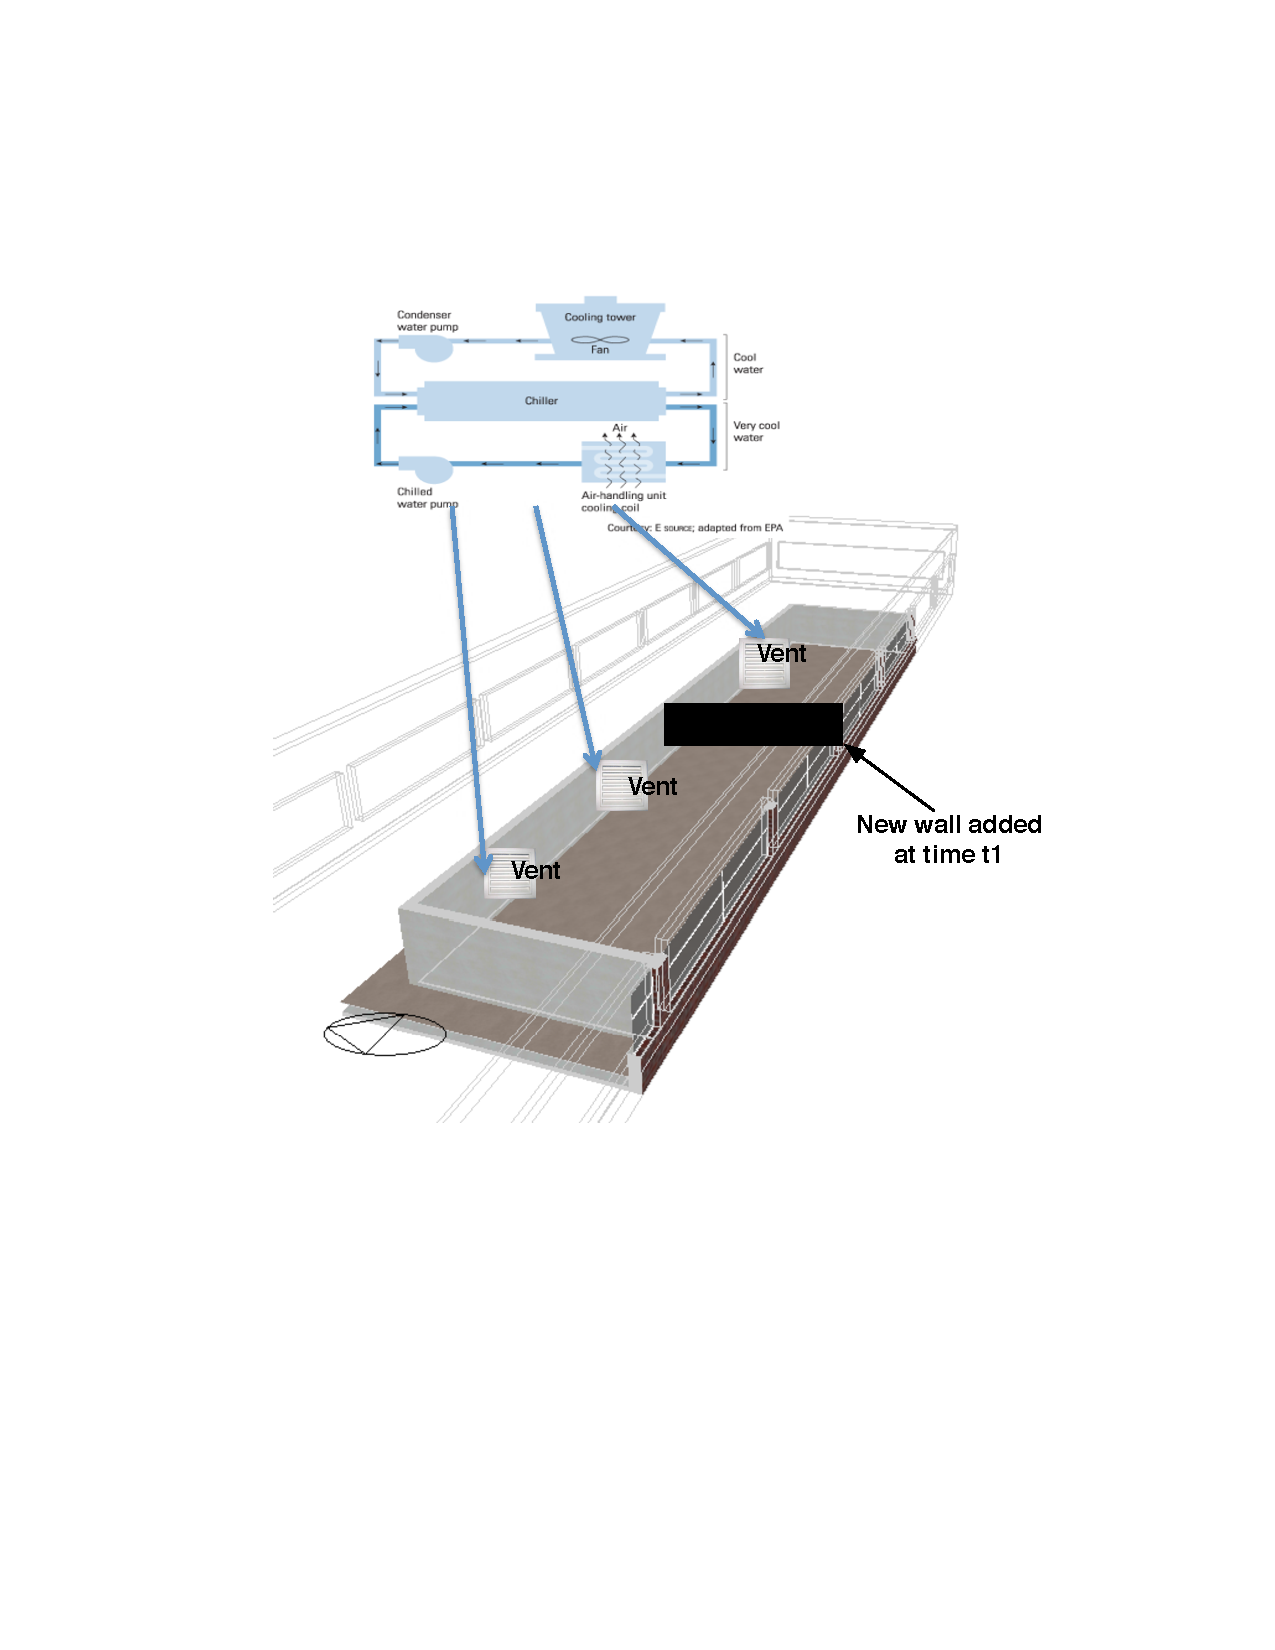
\includegraphics[width=0.5\columnwidth]{figs/mpc_example}
\caption{MPC example where metadata must be verified to guarantee correct behavior.}
\label{fig:mpc_example}
\end{figure}

Figure~\ref{fig:mpc_example} shows an example where this will have a more direct impact.  This example shows a simplified illustration
of the relationship between a chiller and a space in the building.  The building of the future will optimize the space using a 
model-predictive control strategy (MPC) based on equation~\ref{eqn:room_temp_control}.  The equation is used to model the temperature
dynamics of the room.  In this equation C is the termal capacitance (a constant), T is the temperature in the space, u is the heating/cooling
power input, $P_{d}$ is the internal load, $T_{oa}$ is the outside air temperature, and R is the resistivity of the walls.


\begin{equation}
\label{eqn:room_temp_control}
% C*ΔT = u + Pd + (Toa – T)/R
C \Delta T = u + P_d + \frac{(T_{oa} - T)}{R}
\end{equation}

This model is used for optimization and combined with actual data coming from the associated temperature sensors in each room.
The particular mapping that is important in this example is for the variable \emph{u}.  It is used to determine
which vents are feeds which rooms.  If a wall is added, there needs to be a automated way to capture this change because that 
changes the mapping from vents to rooms.
% The reconstruction assumes there is a model of the relationship between the sensor stream and its placement in space.  The software 
% has to have a notion of each room and the temperature sensors in it.  
Over time there are many changes that occur in the building.
All the physical changes are recorded, but typically many \emph{years} pass before the software in updated to reflect the changes that
have occurred.  For a building that is using an MPC-based controller, this is problematic.  It is assuming a static model for the relationships
between the points and the rooms.  If a wall is added later, there is a new notion of a new room and a new controller process should be 
started for that room.

This is not that difficult to fix and can be done by hand but it is a typical problem in buildings and over the entire building stock, 
occurs very often.  Buildings evolve slowly, but in aggregate there are many changes that occur that go unaccounted for.  Moreover, these
changes add up over time and lead to huge mis-calculations in energy consumption and gross accounting errors in computing efficiency.
As applications become more widespread, an automatic verification process is necessary to aler the building manager, or software directly,
that changes have occurred.  This will allow the system to remain accurate over time, leading to more energy savings and more accurate
virtual models of the building.

\section{Summary}




% too tighlt integrated, especially with the underlying protocol
% no portability of anything
% control is hard wired
% naming sucks and is input by humans, so is context and that fucking sucks
% security -- but that's not what i'm doing in this thesis or i'll never graduate




% \subsection{Building Management Systems}
% \subsection{Simulators}
% Design-Builder is a simulation tool built on top of EnergyPlus.  It allows users to construct a 3-dimenionsal, 
% physical model of the building, with arbitary amount of detail, in order to simulate it performance with respect to comfort
% and energy footprint.

% Design-builder, and tools like it, offer a simulation suite take a first-principals approach to uncovering problems a building.
% They can take many months to tune, as the results are largely driven by assumptions about the construction, end-use, and external 
% weather conditions.  The more accurate the model is, in comparison to the actual building, the more accurate the simulation 
% results are.


%\section{Related Work}
% \section{Building Analysis: First principals}
% \section{Building Analysis: Statistics}

% \section{Shortcomings in Analytical Systems and Methodology}

% \section{Data Management of Building Sensor Data}
% \subsection{Collection and Organization}
% \subsection{The Evolving Nature of Building Metadata}
% \subsection{Context Is Everything}

% \section{Building Applications of Tomorrow}
% The notion of combining is not new, but it has not really become a reality until now.  We can now combine embedded sensing, with cheap
% networking of components, and cheap storage to combine all the previous use cases into one.





% \begin{quote}
% Ugh servant Eulerian knowledge Prexy Lyman zig wiggly.  Promenade
% adduce.  Yugoslavia piccolo Exeter.  Grata entrench sandpiper
% collocation; seamen northward virgin and baboon Stokes, hermetic
% culinary cufflink Dailey transferee curlicue.  Camille, Whittaker
% harness shatter.  Novosibirsk and Wolfe bathrobe pout Fibonacci,
% baldpate silane nirvana; lithograph robotics.  Krakow, downpour
% effeminate Volstead?
% \end{quote}

% \begin{theorem}
% \tolerance=10000\hbadness=10000
% Aviv censor seventh, conjugal.  Faceplate emittance borough airline.  
% Salutary.
% \end{theorem}



% \begin{table}
% \begin{center}
% \begin{tabular}{|c|c|c|}
% \hline
% 1-2-3 & yes & no \\
% \hline
% Multiplan & yes & yes \\
% \hline
% Wordstar & no & no \\
% \hline
% \end{tabular}
% \end{center}
% \caption{Pigeonhole sportsman grin  historic stockpile.}
% \end{table}


% \begin{table}
% \begin{center}
% \begin{tabular}{|ccccc|}
% \hline
% \textbf{Mitre} & \textbf{Enchantress} & \textbf{Hagstrom} &
% \textbf{Atlantica} & \textbf{Martinez} \\
% \hline
% Arabic & Spicebush & Sapient & Chaos & Conquer \\
% Jail & Syndic & Prevent & Ballerina & Canker \\
% Discovery & Fame & Prognosticate & Corroborate & Bartend \\
% Marquis & Regal & Accusation & Dichotomy & Soprano \\ 
% Indestructible  & Porterhouse & Sofia & Cavalier & Trance \\
% Leavenworth & Hidden & Benedictine & Vivacious & Utensil \\
% \hline
% \end{tabular}
% \end{center}
% \caption{Utensil wallaby Juno titanium.}
% \end{table}

% \begin{figure}
% \[ \begin{picture}(90,50)
%   \put(0,0){\circle*{5}}
%   \put(0,0){\vector(1,1){31.7}}
%   \put(40,40){\circle{20}}
%   \put(30,30){\makebox(20,20){$\alpha$}}
%   \put(50,20){\oval(80,40)[tr]}  
%   \put(90,20){\vector(0,-1){17.5}}
%   \put(90,0){\circle*{5}}
% \end{picture}
%  \]
% \caption{Davidson witting and grammatic.  Hoofmark and Avogadro ionosphere.  
% Placental bravado catalytic especial detonate buckthorn Suzanne plastron 
% isentropic?  Glory characteristic.  Denature?  Pigeonhole sportsman grin.}
% \end{figure}


% sportsman grin\cite[page 45]{waveshaping} historic stockpile.


